\chapter{Исследовательская часть}
\section{Технические характеристики}
Тестирование выполнялось на устройстве со следующими техническими характеристиками:
\begin{itemize}
	\item Операционная система Pop!\_OS 22.04 LTS \cite{ubuntu} Linux \cite{linux};
	\item Оперативная память 16 GiB;
	\item Процессор AMD® Ryzen 7 2700 eight-core processor × 16 \cite{amd}.
\end{itemize}
Во время тестирования устройство было подключено к блоку питания и не нагружено никакими приложениями, кроме встроенных приложений окружения, окружением и системой тестирования.

\section{Демонстрация работы программы}



На рисунке \ref{demonstration} представлен результат работы программы.

\begin{figure}[ht!]
	\begin{center}
		\captionsetup{singlelinecheck = false, justification=centerfirst}
		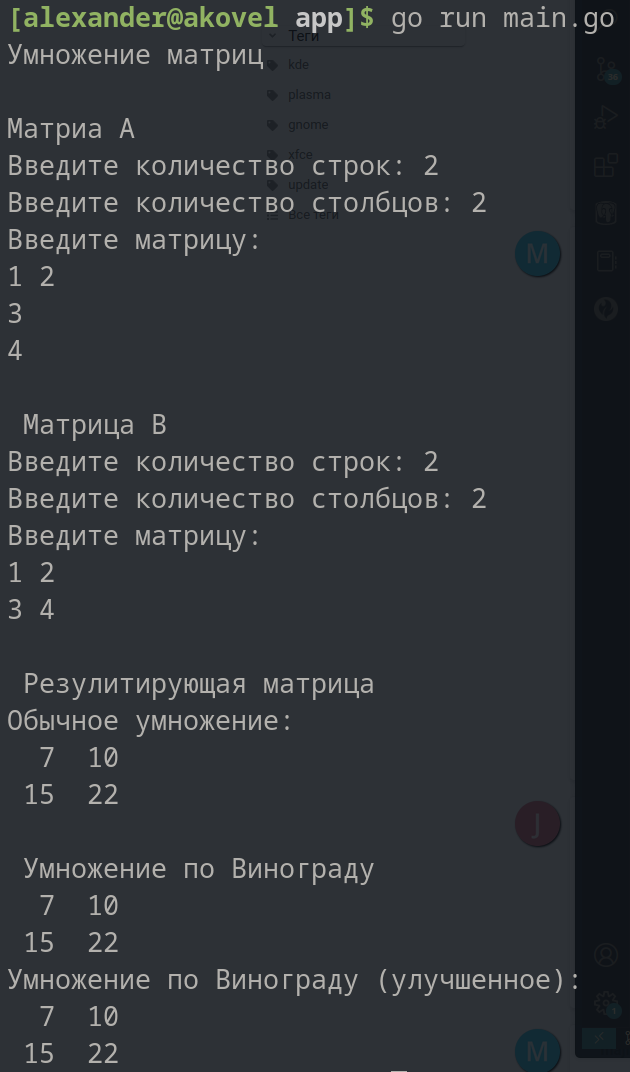
\includegraphics[scale=0.5]{assets/demonstration.png}
		\caption{Пример работы программы}
		\label{demonstration}
	\end{center}
	
	
\end{figure}

\newpage

\section{Время выполнения алгоритмов}

Алгоритмы тестировались при помощи вставки кода на языке СИ \ref{bench}. Данная команда возвращает значения процессорного времени типа int в наносекундах.

Замеры времени для каждого алгоритма проводились 100 раз.

\begin{lstlisting}[label=bench,caption=Пример теста эффективности]
	/*
	#include <pthread.h>
	#include <time.h>
	#include <stdio.h>
	
	static long long getThreadCpuTimeNs() {
		struct timespec t;
		if (clock_gettime(CLOCK_THREAD_CPUTIME_ID, &t)) {
			perror("clock_gettime");
			return 0;
		}
		return t.tv_sec * 1000000000LL + t.tv_nsec;
	}
	*/
	import "C"	
	
	func test(){
		
		cputime1 := C.getThreadCpuTimeNs()
		for i := 0; i < n; i++ {
			matrix.WinogradMult(amat, bmat)
		}
		cputime2 := C.getThreadCpuTimeNs()
		fmt.Printf(cputime2 - cputime1)
		
	}
\end{lstlisting}

Результаты профилирования алгоритмов приведены в таблице \ref{tab:time}. Результаты тестирования приведены в таблице \ref{table:testing}.
\begin{table}[ht!]
	\captionsetup{singlelinecheck = false, justification=raggedleft}
	\caption{Время выполнения алгоритмов}
	\renewcommand{\arraystretch}{1.4}
	\begin{subtable}[ht!]{0.45\textwidth}
		\centering
		\caption{Четная размерность матриц}
		\begin{tabular}{||l|l|l|l||}
			\hline
			\multirow{2}{*}{n} & \multicolumn{3}{l||}{Время, ns} \\ \cline{2-4} 
			&  Класс. & Виноград & Вин. опт. \\ \hline\hline
			10 & 4.49e-06 & 3.91e-06 & 4.01e-06 \\ \hline 
			20 & 2.74e-05 & 2.24e-05 & 2.30e-05 \\ \hline 
			30 & 8.84e-05 & 6.72e-05 & 7.01e-05 \\ \hline 
			40 & 2.09e-04 & 1.49e-04 & 1.58e-04 \\ \hline 
			50 & 3.96e-04 & 2.98e-04 & 3.14e-04 \\ \hline 
			60 & 6.58e-04 & 4.95e-04 & 5.15e-04 \\ \hline 
			70 & 1.07e-03 & 7.95e-04 & 8.43e-04 \\ \hline 
			80 & 1.60e-03 & 1.20e-03 & 1.22e-03 \\ \hline 
			90 & 2.26e-03 & 1.68e-03 & 1.77e-03 \\ \hline 
			100 & 3.14e-03 & 2.25e-03 & 2.38e-03 \\ \hline 
			150 & 1.06e-02 & 7.88e-03 & 8.33e-03 \\ \hline 
			200 & 2.84e-02 & 2.20e-02 & 2.34e-02 \\ \hline 
			250 & 6.73e-02 & 5.34e-02 & 5.74e-02 \\ \hline 
			300 & 1.14e-01 & 8.97e-02 & 9.60e-02 \\ \hline 
			350 & 1.80e-01 & 1.39e-01 & 1.50e-01 \\ \hline 
			400 & 2.67e-01 & 2.05e-01 & 2.21e-01 \\ \hline 
			450 & 4.17e-01 & 3.23e-01 & 3.48e-01 \\ \hline 
			500 & 5.71e-01 & 4.42e-01 & 4.75e-01 \\ \hline 
		\end{tabular}
		\label{tab:odd}
	\end{subtable}
	\hfill
	\begin{subtable}[ht!]{0.45\textwidth}
		\centering
		\caption{Нечетная размерность матриц}
		\begin{tabular}{||l|l|l|l||}
			\hline
			\multirow{2}{*}{n} & \multicolumn{3}{l|}{Время, ns} \\ \cline{2-4} 
			&  Класс. & Виноград & Вин. опт. \\ \hline\hline
			11 & 5.17e-06 & 4.56e-06 & 5.05e-06 \\ \hline 
			21 & 3.25e-05 & 2.58e-05 & 2.59e-05 \\ \hline 
			31 & 9.63e-05 & 7.23e-05 & 7.69e-05 \\ \hline 
			41 & 2.14e-04 & 1.64e-04 & 1.73e-04 \\ \hline 
			51 & 4.10e-04 & 3.15e-04 & 3.38e-04 \\ \hline 
			61 & 7.13e-04 & 5.37e-04 & 5.70e-04 \\ \hline 
			71 & 1.11e-03 & 8.36e-04 & 8.79e-04 \\ \hline 
			81 & 1.67e-03 & 1.28e-03 & 1.35e-03 \\ \hline 
			91 & 2.33e-03 & 1.73e-03 & 1.85e-03 \\ \hline 
			101 & 3.23e-03 & 2.36e-03 & 2.49e-03 \\ \hline 
			151 & 1.08e-02 & 8.03e-03 & 8.50e-03 \\ \hline 
			201 & 2.74e-02 & 2.13e-02 & 2.29e-02 \\ \hline 
			251 & 6.80e-02 & 5.27e-02 & 5.66e-02 \\ \hline 
			301 & 1.16e-01 & 9.13e-02 & 9.82e-02 \\ \hline 
			351 & 1.82e-01 & 1.40e-01 & 1.52e-01 \\ \hline 
			401 & 2.58e-01 & 1.99e-01 & 2.14e-01 \\ \hline 
			451 & 4.21e-01 & 3.26e-01 & 3.50e-01 \\ \hline 
			501 & 5.74e-01 & 4.43e-01 & 4.76e-01 \\ \hline 
		\end{tabular}
		\label{tab:even}
	\end{subtable}
	\label{tab:time}
\end{table} 

\newpage

\section{Графики функций}


\begin{figure}[ht!]
	\captionsetup{singlelinecheck = false, justification=centering}
	\centering
	\begin{subfigure}[b]{\textwidth}
		\centering
		\begin{tikzpicture}
			\begin{axis}[
				xlabel={размер матрицы},
				ylabel={время, ns},
				width = 0.95\textwidth,
				height=0.3\textheight,
				xmin=0, xmax=600,
				legend pos=north west,
				xmajorgrids=true,
				grid style=dashed,
				]
				\addplot[
				color=blue,
				mark=asterisk,
				]
				table {assets/cw-ev.dat};
				\addplot[
				color=red,
				mark=o,
				]
				table {assets/o-cw-ev.dat};
				\legend{Неоптимизированный, Оптимизированный}
			\end{axis}
		\end{tikzpicture}
		\caption{Четная размерность матрицы}
	\end{subfigure}
	\hfill
	\newline
	\begin{subfigure}[b]{\textwidth}
		\centering
		\begin{tikzpicture}
			\begin{axis}[
				xlabel={размер матрицы},
				ylabel={время, ns},
				width = 0.95\textwidth,
				height=0.3\textheight,
				xmin=0, xmax=600,
				legend pos=north west,
				xmajorgrids=true,
				grid style=dashed,
				];
				
				\addplot[
				color=blue,
				mark=asterisk,
				]
				table {assets/cw-odd.dat};
				\addplot[
				color=red,
				mark=o,
				]
				table {assets/o-cw-odd.dat};
				\legend{Неоптимизированный, Оптимизированный}
			\end{axis}
		\end{tikzpicture}
		\caption{Нечетная размерность матрицы}
		\label{fig:w-plot}
	\end{subfigure}
	\hfill
	
\end{figure}

\clearpage

\section*{Вывод}

В данном разделе были сравнены алгоритмы по времени.
Оптимизированный алгоритм Винограда является самым быстрым, за счет проведенных изменений в стандартном алгоритме Винограда.
